%SourceDoc ../YourName-Dissertation.tex
\chapter{Introduction} \label{chapter1:introduction}

\section{\sloppy Organic Polymers for Optical Applications}

Organic polymers are emerging materials that feature many attractive properties compared to conventional inorganic materials. Devices made out of organic polymers are generally flexible, mechanically stable on impact, light-weight, and inexpensive to produce. This has led to increased efforts in utilizing these compounds in many different application domains, which include optic and optoelectronic devices such as organic light-emitting diodes \cite{ThejoKalyani2012}, complementary metal oxide semiconductor \cite{Nakagawa2010}, photovoltaics \cite{Hachmann2011}, field-effect transistors \cite{Sirringhaus2009}, displays, and image sensors \cite{Angione2011}. In these devices, they can be introduced \insitu\ as microlenses, waveguides, microresonators, interferometers, anti-reflective coatings, optical adhesives, and substrates (see Fig. \ref{fig:HRIP_apps}).
Most of these applications require materials with superior optical properties (such as high RI values). While typical carbon-based polymers exhibit poor optical properties when compared to inorganic materials \cite{Liu2009}, an important advantage of organic materials is that their properties can be tuned readily and significantly by controlling their molecular structure. Thus, organic materials are a prime example for a rational design target.
%%%
\begin{figure}[htbp]
\centering
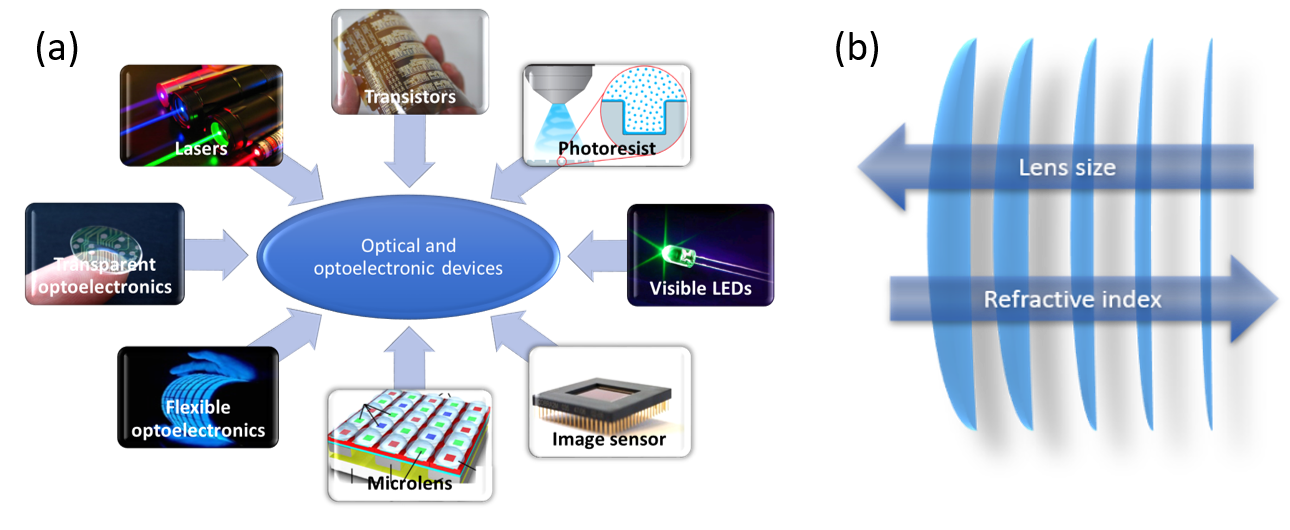
\includegraphics[width=0.95\textwidth]{Chapter-1/Figures/HRIP_apps.png}
\caption{\textbf{(a)} Application range of organic polymers in optoelectronics. \textbf{(b)} Relationship of RI value and lens thickness.}
\label{fig:HRIP_apps}
\end{figure}
%%%

%The traditional, experimentally focused discovery process for new materials is very time-, labor-, and resource-intensive, which limits the number and diversity of candidate compounds that can be explored. 
The two principal challenges in creating new chemistry and materials are that their behavior is governed by complicated structure-property and structure-activity relationships \cite{Selassie2003,Muller2005,LeBaillydeTilleghem2007}, and that chemical space is practically infinite \cite{Lipinski2004,Kirkpatrick2004,Dobson2004}. 
Traditional experiment-driven trial-and-error approaches are increasingly ill-equipped to meet these challenges on their own, in particular since advanced systems require more and more intricate property profiles \cite{Zvinavashe2008,Scior:2009-11,Schneider2010}. 
Progress thus tends to be slow and incremental, in particular for advanced materials systems, which require more and more intricate property profiles. However, chemical and materials research has been undergoing a significant transformation in recent years that can alleviate many of these shortcomings: After decades of continuous advances in methods, algorithms, and computer hardware, the fields of modeling and simulation have reached a tipping point, and they are finally at a stage where they can make accurate predictions for systems that are both realistic and relevant. Progress is now increasingly driven by computational studies, which have become crucial assets in the pursuit of next-generation materials and chemistry. By making guiding predictions, they can significantly boost the efficiency of research endeavors, and uncover promising targets for investigations in the laboratory (see, \eg  Ref.\ \cite{cep01,Sokolov2011,Hachmann2011,Olivares-Amaya2011,Amador-Bedolla2013,Hachmann2014,Pyzer-Knapp2015,Lopez2016}). The White House Materials Genome Initiative (MGI) \cite{NationalMaterials2011} underscores the value of integrated joint ventures between experimentalists and theoreticians in tackling complex discovery and design challenges and delivering revolutionary new materials. That being said, the usual focus on individual compounds has so far been limiting the utility of computational research. While there is obvious value in characterizing particular systems of interest, the insights gained in these small-scale studies cannot easily be transferred or generalized.

Our group is developing a data-driven and rational design framework for accelerating the discovery and design of new chemicals/materials. In this dissertation, I deploy this framework to identify new polymer systems with superior optical properties, specifically the high-refractive-index polymers (HRIPs).


\section{Data-Driven Design of Chemical Systems and the Exploration of Chemical Space}

% introduce data-driven research; point to MGI and other high-profile initiatives for support of promise 
The shift towards a data-driven discovery and rational design paradigm (cf.\ Fig.\ \ref{fig:4th_pillar}) promises to mitigate many of the inefficiencies and shortcomings that are still prevalent in contemporary chemical research. 
% point to MGI and other high-profile initiatives as authorities for support of premise 
There is now a growing agreement on the value of incorporating modern data science -- the 4th pillar of science -- into chemical research, and this development has been recognized by high-profile funding programs such as the MGI \cite{NationalMaterials2011}.
% explain problem setting 
Yet, despite impressive pioneering efforts (\eg  \cite{Hansen2013a,Huan2015,PhysRevB.87.219902,doi:10.1021/cm503507h,Behler2007}), 
there is still a distinct disconnect between the promise of this approach and the realities of every-day research in the chemistry community, where data-driven work does not yet play a significant role. 

\begin{figure}[htbp]
	\centering
	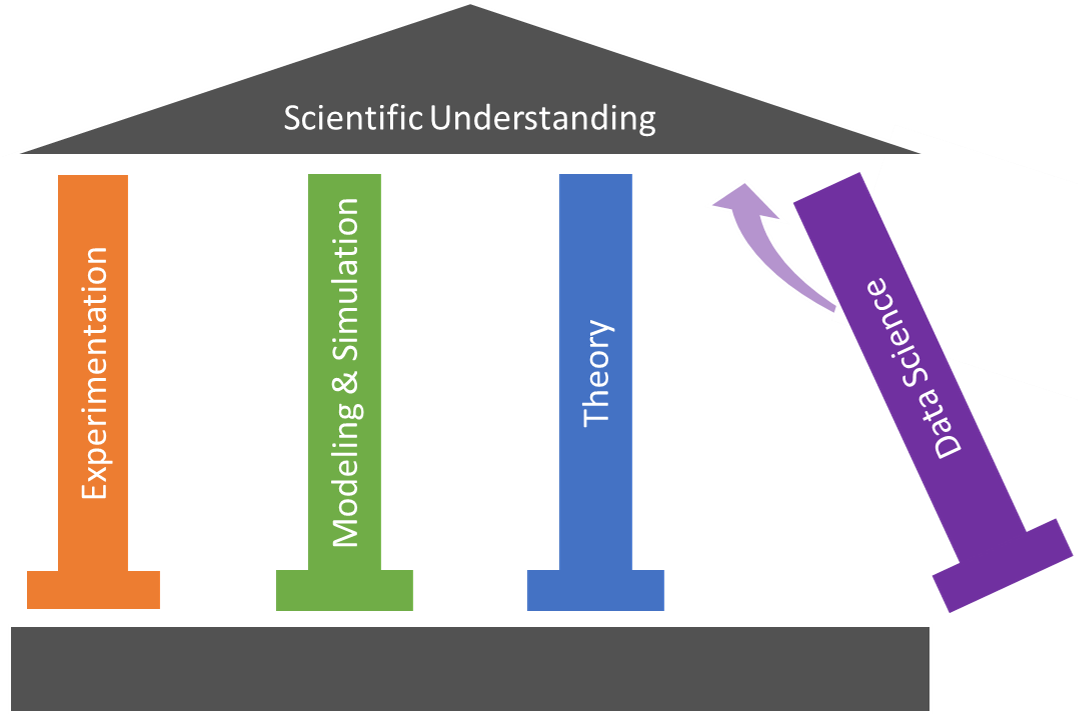
\includegraphics[width=0.7\textwidth]{Chapter-1/Figures/4th_pillar.png}
	\caption{The rise of data science as the 4th pillar of science.}
	\label{fig:4th_pillar}
\end{figure}

\subsection{Group's Approach for Data-Driven \textit{In Silico} Research}
%% Copied from the Molecular Simulation paper
We have developed a basic template for data-driven \insilico\ research, which addresses the inherent challenges in the discovery and design of new chemistry, in particular as part of integrated joint ventures with experimentalists. It provides the foundation and framework for our research program, and its rationale can be summarized as following: 
\begin{itemize}
	\item Using computational modeling and simulations, we can rapidly and efficiently assess the properties, behavior, and performance potential of candidate compounds, materials, and/or chemical transformations for a given problem setting \cite{Olivares-Amaya2011,Wen2012,Stevanovic2014}.
	\item By combining modeling and simulation with high-throughput screening techniques, we can characterize candidates on a massive scale. These studies naturally lead to big data scenarios \cite{Potyrailo2011,Hachmann2011,Hachmann2014,Gunter2012,White2013}.
	\item Using modern database technology, we can readily store and access the resulting data sets, \eg  to identify candidates with desired property combinations for on-demand applications \cite{Blum2011,Ruddigkeit2012}.
	\item In addition to the immediate information obtained for these thousands or even millions of candidates, we can mine the generated data in its entirety. Using machine learning, we can gain insights into the mechanisms that determine their characteristics and cast these findings into predictive models \cite{Rupp2012,Pilania2013,Mansbach2015}.
	\item By identifying these design rules as well as high-value moieties, building blocks, structural patterns, or more general features, we can accomplish the \denovo\ design of next-generation candidates \cite{Pegg2001,Proschak2009,Nakamura2012}. Using the predictive models, we can conduct hyperscreenings, \ie screenings based on data-derived models that typically surpass the scale of the original screenings (based on physics-derived models) by several orders of magnitude.
	\item Experimentalist partners can pursue the top candidates from the (hyper-)screening and/or \denovo\ design. This guidance allows the experimentalists to focus on highly promising targets and avoid wasted efforts on unpromising ones \cite{Sokolov2011}. Additional in-depth modeling and simulations can contribute further insights to the experimental findings, which allow for the advanced optimization of lead candidates. 
	\item The experimental results can be included as training data in the machine learning approaches. In addition, they can be used to validate, benchmark, calibrate, and potentially improve the physics-based modeling and simulation protocols, which closes the design loop \cite{Hartenfeller2011a}. 
\end{itemize}

\subsection{Software Ecosystem for Materials Discovery}

Our group has identified four components that are critical for the efficient discovery of materials with targeted properties. These four components are being developed in the group as four different software packages (see Fig.\ \ref{fig:ecosystem}):
 
\begin{figure}[htbp]
	\centering
	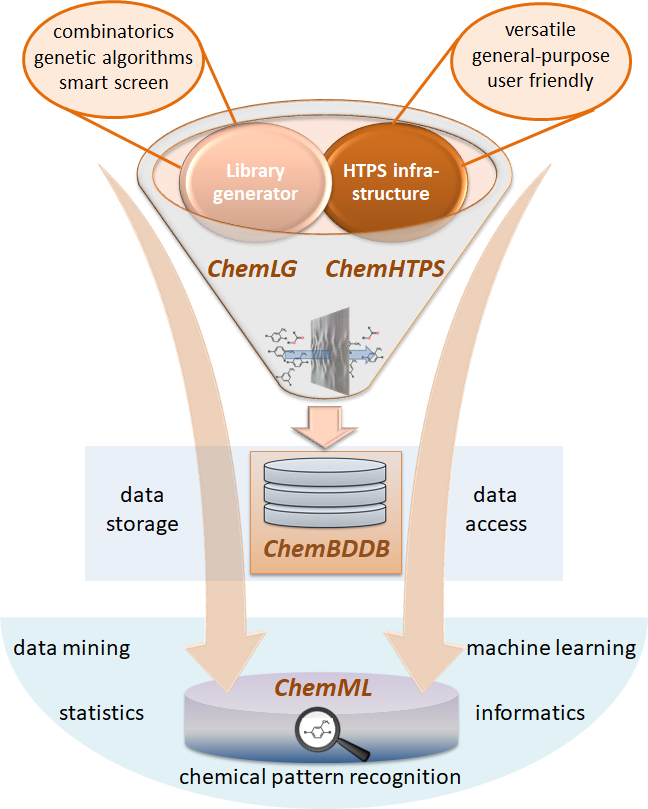
\includegraphics[width=0.6\textwidth]{Chapter-1/Figures/ecosystem.png}
	\caption{Schematic and connectivity of the software ecosystem comprised of the \chemlg , \chemhtps , \chembddb , and \chemml\  codes.}
	\label{fig:ecosystem}
\end{figure}

\begin{enumerate}
	\item \textbf{\chemlg: Screening library generator \cite{Afzal2018b}.} A prerequisite for the high-throughput exploration of chemical space is access to suitable, large-scale screening libraries. We have developed a corresponding generator for compound and material candidate libraries. We discuss in detail the underlying concepts of \chemlg\ in the Chapter 4 and provide case studies where \chemlg\ was successfully applied. I developed \chemlg\ primarily for the creation of high RI polymer candidates.
	\item \textbf{\chemhtps: Virtual high-throughput screening infrastructure \cite{Afzal2018c}.}  \chemhtps\ is a suite for performing large-scale simulations on high-performance computing clusters. This suite supports various quantum chemistry and molecular modeling codes including Q-Chem, ORCA, GROMACS, and LAMMPS. I co-developed \chemhtps\ infrastructure along with William Evangelista. 
	\item \textbf{\chembddb: Database infrastructure \cite{Shirish2018}.} The use of modern databases is of particular importance in the context of data-intensive research. Despite their great utility and despite being essential for projects that accumulate large data sets, they are still rarely employed in chemical research. Our group has developed a database platform to store and provide access to the various results in a centralized fashion. The database also serves as the focal point for the information exchange within the project team and potential external collaborators, as well as for the coordination of the different project components. The developers of \chembddb\ are Aditya Sonpal and Shirish Sivaraj.
	\item \textbf{\chemml: Data analysis, mining, and modeling infrastructure \cite{Haghighatlari2017}.}  \chemml\ suite includes data analysis, mining, and modeling capabilities that allow us to apply state-of-the-art machine learning and informatics methodology to chemical and materials data sets. Using \chemml, we can identify underlying structure-property relationships which are key to create new and more targeted candidate libraries. The primary developer of \chemml\ is Mojtaba Haghighatlari.
	
\end{enumerate}


\subsection{Discovery of High-Refractive-Index Polymers}

Harnessing the potential of organic polymers in optical and optoelectronic industries has been quite limited because these applications require materials to have RI greater than 1.7, while carbon-based polymers inherently have RIs between 1.3 and 1.5. As a result, there is an incentive to discover new high-refractive index polymers for the aforementioned applications. According to the Lorentz-Lorenz equation, the incorporation of substituents with a high molar refractivity and low molar volume can increase the RI values of these materials. This suggests that the ability to tailor the molecular structure of polymers is the key to increasing their RI values \cite{Liu2009}. On the other hand, tailoring the structure using different functional groups could potentially lead to an infinite number of molecular candidates. It is impractical to empirically characterize a large number of candidates, whereas computational analysis allows greater exploration at a mere fraction of the time and cost. The current work is concerned with creating fast and accurate predictive models for the optical properties of organic polymers, which will guide our experimentalist partners and allow them to target the most promising candidates. The application of above mentioned rational design framework in the current work has allowed us to accelerate the discovery of polymers with high RI values materials.

We have developed an accurate model for the prediction of RI values of polymers based on \firstprinciples\ and molecular modeling techniques. The model is based on the Lorentz-Lorenz equation and thus includes the calculation of polarizability and number density values for the candidate structures. In this scheme, we compute the molecular polarizability using \firstprinciples\ electronic structure theory (DFT) and the number density using molecular modeling (MD). The synergistic combination of DFT and MD resulted in a successful and economical model for RI prediction. We validated the RI model using experimental RI values of 112 non-conjugated polymers, which shows that the model is in a good agreement ($R^2$=0.94) with the experimental results \cite{Afzal2018a}. Further details of the model and its validation will be discussed in Chapter 2.

In the RI prediction model, we apply computationally expensive DFT computations. While the choice proved remarkably successful, it represents the bottleneck step in our RI protocol due to computational inefficiency. It thus limits the utility of the overall approach, particularly in the context of virtual high-throughput screenings of large-scale candidate libraries. Therefore, we have systematically benchmarked several DFT model chemistries to find one that optimizes the balance between accuracy and efficiency in the target compounds space. We further compare the results for non-conjugated and conjugated polymers, offer guidance for method selection, and analyze the errors that propagate into the RI predictions. We will discuss the details of the benchmarking study in Chapter 3. 

In search of candidates with high RI values, we created a library of polymers using the \chemlg\ software. In this work, we selected polyimides as a model polymer and created a library of novel polyimides based on the building blocks suggested by our experimental collaborators. We provide an exposition of \chemlg\ software package in chapter 4. The resultant library of polyimides consists of 270,000 candidates. Application of our rational design framework resulted in more than 2000 polyimides with RI values greater than 1.8. The results from the study are presented in Chapter 5.

A large-scale exploration of chemical space will not only identify exceptional molecular targets but also allow us to identify underlying patterns and global trends. These structure-property relationships can aid in the inverse design of materials with specific properties. To achieve this, we created a massive library of 1.5 million small organic molecules and evaluated their properties. Characterization of candidates on such a large scale was possible by the application of advance machine learning techniques. Using the big data obtained form this work, we identified design rules as well as high-value building blocks, and structural patterns that correlate with optical properties. Additionally, we uncovered regions in chemical space where we can maximize the optical properties of organic molecules. These guidelines allow us to target specific molecular motifs and create the next generation of materials with exceptional properties. We present the results from this large-scale exploration in Chapter 6.

This dissertation demonstrates that the developed rational design framework is a powerful tool. The exploration of high-refractive-index polymers is one example for applications problems and I spearheaded this project as part of my dissertation.
